\chapter{Analisis}
\label{chap:analisis}

Pada bab ini akan dibahas analisis terhadap teori-teori yang telah dibahas sebelumnya. Analisis akan meliputi studi kasus untuk penerapan metode \textit{secret sharing} Shamir, pemilihan \begin{math}n\end{math} dan \begin{math}k\end{math}, dan perancangan perangkat lunak.

\section{Studi Kasus}

Pada bagian ini akan dibahas studi kasus tentang bagaimana penerapan metode \textit{secret sharing} Shamir untuk banyak password. Studi kasus meliputi pengenalan kasus, pembangunan share, dan rekonstruksi rahasia.

\subsection{Pengenalan Kasus}\label{subsec:pengenalankasus}

Langkah awal yang dibutuhkan untuk mengembalikan banyak \textit{password} dengan metode \textit{secret sharing} Shamir, diperlukan beberapa tahap proses. Proses pertama adalah proses penyimpanan \textit{password}. Kemudian, proses selanjutnya adalah proses untuk mengembalikan banyak \textit{password}. Proses pertama membutuhkan beberapa \textit{password}. Untuk \begin{math}n\end{math} buah \textit{password}, maka akan dibuat \begin{math}n\end{math} buah pertanyaan keamanan. Sementara itu, untuk proses mengembalikan \textit{password} dibutuhkan pertanyaan keamanan yang sudah dibuat dalam proses sebelumnya.

Untuk kedua proses di atas, diasumsikan banyak \textit{password} yang akan disimpan sebanyak 5 buah. Setiap \textit{password} akan diberi label \begin{math}p_1\end{math}, \begin{math}p_2\end{math}, sampai \begin{math}p_5\end{math}. Persamaan \ref{eq:passwords1} sampai \ref{eq:passwords5} menunjukkan \begin{math}p_1\end{math} sampai \begin{math}p_5\end{math}.

\begin{gather}
	p_1 = 123456 \label{eq:passwords1} \\
	p_2 = password \label{eq:passwords2} \\
	p_3 = hello123 \label{eq:passwords3} \\
	p_4 = secret \label{eq:passwords4} \\
	p_5 = foobar \label{eq:passwords5}
\end{gather}

\subsection{Proses Penyimpanan \textit{Password}}\label{subsec:simpanpassword}

Proses penyimpanan \textit{password} dibagi menjadi 2 proses, yaitu proses pembangunan \textit{share} untuk masing-masing \textit{password} dan proses enkripsi dari setiap \textit{share} yang sudah dibangun. Pada bagian ini akan dibahas kedua proses tersebut.

\subsubsection{Proses Pembangunan \textit{Share}}

Pada proses ini, akan dilakukan pembangunan \textit{share} dari masing-masing \textit{password}. Langkah-langkah untuk membangun share adalah sebagai berikut.

\begin{enumerate}
	\item Membagi setiap \textit{password} \begin{math}p_i\end{math} menjadi beberapa karakter, masing-masing karakter akan diubah menjadi nilai ASCIInya, \begin{math}c_1, c_2, ..., c_m\end{math}.
		\item Memilih nilai \begin{math}n\end{math}, yaitu banyak \textit{share} yang akan dibangun.
	\item Memilih nilai \begin{math}k\end{math}, yaitu banyak minimal pertanyaan keamanan yang harus dijawab dengan benar, dimana \begin{math}0 < k \leq n\end{math}.
	\item Memilih \begin{math}k-1\end{math} angka acak, \begin{math}d_1, d_2, ..., d_{k-1}\end{math}, untuk masing-masing karakter \begin{math}c_1, c_2, ..., c_m\end{math}.
	\item Membentuk fungsi \begin{math}f_m(x)\end{math} untuk masing-masing karakter \begin{math}c_1, c_2, ..., c_m\end{math}. 
	Komponen dari fungsi \begin{math}f_m(x)\end{math} terdiri atas \begin{math}c_m\end{math} sebagai konstanta tanpa koefesien, \begin{math}d_1, d_2, ..., d_{k-1}\end{math} sebagai konstanta dengan koefesien. Persamaan \ref{eq:fungsifx} menunjukkan persamaan dari fungsi \begin{math}f_m(x)\end{math} yang harus dibentuk.
	\begin{equation}
		f_m(x) = c_m + d_1x + d_2x^2 + d_3x^3 + ... + d_{k-1}x^{k-1}
		\label{eq:fungsifx}
	\end{equation}
	\item Menghitung masing-masing nilai \begin{math}x\end{math} dari \begin{math}x=1, x=2, ..., x=n\end{math} untuk fungsi \begin{math}f_m(x)\end{math}.
	\item Nilai \begin{math}f_m(1)\end{math} sampai \begin{math}f_m(n)\end{math} adalah nilai \textit{share} untuk password \begin{math}p_i\end{math}.
\end{enumerate}

Kembali kepada kasus pada Subbab \ref{subsec:pengenalankasus}, misalkan \textit{password} yang akan dibangun \textit{share-share}nya adalah \begin{math}p_1\end{math}. Langkah pertama adalah membagi \begin{math}p_1\end{math} menjadi beberapa karakter dan mengubah masing-masing karakter menjadi nilai ASCIInya. Persamaan \ref{eq:ubahascii1} sampai \ref{eq:ubahascii7} menunjukkan langkah pertama.

\begin{gather}
	p_1 = 123456 \label{eq:ubahascii1} \\
	c_1 = '1' = 49 \label{eq:ubahascii2} \\
	c_2 = '2' = 50 \label{eq:ubahascii3} \\
	c_3 = '3' = 51 \label{eq:ubahascii4} \\
	c_4 = '4' = 52 \label{eq:ubahascii5} \\
	c_5 = '5' = 53 \label{eq:ubahascii6} \\
	c_6 = '6' = 54 \label{eq:ubahascii7}
\end{gather}

Langkah selanjutnya adalah memilih nilai \begin{math}n\end{math}. Karena banyak \textit{password} \begin{math}p_i\end{math} adalah 5, maka banyak \textit{share} untuk masing-masing \textit{password} sebanyak 5. Maka, \begin{math}n=5\end{math}.

Setelah memilih nilai \begin{math}n\end{math}, langkah berikutnya adalah memilih nilai \begin{math}k\end{math}. Nilai \begin{math}k\end{math} ini nanti akan berhubungan dengan banyak minimal pertanyaan keamanan yang harus dijawab benar untuk mengembalikan \textit{password}. Untuk kasus ini, dipilih \begin{math}k=3\end{math}.

Langkah selanjutnya adalah memilih \begin{math}k-1\end{math} angka acak untuk masing-masing karakter \begin{math}c_1\end{math} sampai \begin{math}c_6\end{math}. Karena \begin{math}k=3\end{math}, maka dipilih 2 angka acak untuk masing-masing karakter. Berikut angka acak untuk masing-masing karakter.

\begin{itemize}
	\item \begin{math}c_1\end{math}: 12 dan 6.
	\item \begin{math}c_2\end{math}: 15 dan 11.
	\item \begin{math}c_3\end{math}: 22 dan 1.
	\item \begin{math}c_4\end{math}: 21 dan 3.
	\item \begin{math}c_5\end{math}: 19 dan 8.
	\item \begin{math}c_6\end{math}: 25 dan 17.
\end{itemize}

Setelah memilih angka acak untuk masing-masing karakter, langkah selanjutnya adalah membentuk fungsi \begin{math}f(x)\end{math} untuk masing-masing karakter. Maka, fungsi \begin{math}f_1(x)\end{math} sampai \begin{math}f_6(x)\end{math} yang dibentuk adalah sebagai ditunjukkan pada persamaan \ref{eq:fungsi1} sampai \ref{eq:fungsi6}.

\begin{gather}
	f_1(x) = 49 + 12x + 6x^2 \label{eq:fungsi1} \\
	f_2(x) = 50 + 15x + 11x^2 \label{eq:fungsi2} \\
	f_3(x) = 51 + 22x + x^2 \label{eq:fungsi3} \\
	f_4(x) = 52 + 21x + 3x^2 \label{eq:fungsi4} \\
	f_5(x) = 53 + 19x + 8x^2 \label{eq:fungsi5} \\
	f_6(x) = 54 + 25x + 17x^2 \label{eq:fungsi6}
\end{gather}

Langkah selanjutnya adalah menghitung nilai \begin{math}x=1, x=2, ..., x=n\end{math} untuk fungsi \begin{math}f_1(x)\end{math} sampai \begin{math}f_6(x)\end{math}. Tabel \ref{table:itungx} menunjukkan nilai \begin{math}x=1\end{math} sampai \begin{math}x=5\end{math} untuk masing-masing fungsi \begin{math}f(x)\end{math}.

\begin{table}[H]
	\begin{center}
		\caption{Nilai \textit{x} untuk masing-masing \textit{f(x)}}\label{table:itungx}
		\begin{tabular}{| >{$}l<{$} | >{$}l<{$} | >{$}l<{$} | >{$}l<{$} | >{$}l<{$} | >{$}l<{$} | >{$}l<{$} |}
				\hline
				& f_1(x) 	& f_2(x) 	& f_3(x) 	& f_4(x) 	& f_5(x) 	& f_6(x) 	\\ \hline
			1 & 67	 		& 76 			& 74			& 76			& 80			& 96			\\ \hline
			2 & 97 			& 124			& 99			& 106			& 123			& 172			\\ \hline
			3 & 139 		& 194			& 126			& 142			& 182			& 282			\\ \hline
			4 & 193 		& 286			& 155			& 184			& 257			& 426			\\ \hline
			5 & 259 		& 400			& 186			& 232			& 348			& 604			\\ \hline
		\end{tabular}
	\end{center}
\end{table}

Setiap nilai \begin{math}x\end{math} pada Tabel \ref{table:itungx} adalah nilai \textit{share-share} untuk password \begin{math}p_1\end{math}. Setiap nilai \begin{math}x\end{math} ini akan diberi label \begin{math}s_{11}\end{math} untuk \textit{share} pertama dari fungsi pertama, \begin{math}s_{21}\end{math} untuk \textit{share} kedua dari fungsi pertama, dan seterusnya sampai \begin{math}s_{56}\end{math} untuk \textit{share} kelima dari fungsi keenam. Nilai \textit{share} yang sudah diberi label ditunjukkan pada persamaan \ref{eq:nilaishare}.

\begin{equation}
	s_{11} = 67, s_{21} = 97, ..., s_{34} = 155, ..., s_{56} = 604 \label{eq:nilaishare}
\end{equation}

Sementara itu, untuk menghitung nilai share dari \textit{password} \begin{math}p_2\end{math} sampai \begin{math}p_5\end{math}, proses yang sama untuk menghitung \textit{password} \begin{math}p_1\end{math} akan dilakukan. Setelah menghitung nilai \textit{share} untuk \textit{password} \begin{math}p_1\end{math}, langkah selanjutnya adalah proses enkripsi masing-masing \textit{share} ini.

\subsubsection{Proses Enkripsi \textit{Share}}

Pada proses ini, sebelum masing-masing \textit{share} disimpan, masing-masing \textit{share} harus dienkripsi terlebih dahulu. Dalam proses ini juga, \begin{math}n\end{math} buah pertanyaan keamanan akan dibuat. Langkah-langkah proses enkripsi \textit{share} adalah sebagai berikut.

\begin{enumerate}
	\item Membuat \begin{math}n\end{math} pertanyaan keamanan, \begin{math}q_1, q_2, ..., q_n\end{math}.
	\item Menentukan jawaban dari masing-masing pertanyaan keamanan, \begin{math}a_1, a_2, ..., a_n\end{math}.
	\item Menentukan nilai \textit{salt}, \begin{math}r_s\end{math}.
	\item Menghitung \textit{digest} untuk masing-masing konkatenasi dari pertanyaan, jawaban, dan \textit{salt}. Persamaan \ref{eq:itunghash} menunjukkan proses menghitung \textit{digest}.
	\begin{equation}
		h_n = H(q_n + a_n + r_s) \label{eq:itunghash}
	\end{equation}
	\item Setiap nilai \textit{share}, \begin{math}s_{11}, s_{21}, ..., s_{56}\end{math} akan dienkripsi dengan menggunakan digest sebagai kunci. Persamaan \ref{eq:enkripsi} menunjukkan langkah enkripsi \textit{share}.
	\begin{equation}
		E_{h_n}(s_{nm}) = c_{nm}
	\end{equation}
	Pada persamaan \ref{eq:enkripsi}, \begin{math}m\end{math} merupakan banyak karakter dari masing-masing \textit{password} \begin{math}p_i\end{math}.
\end{enumerate}

Kembali kepada kasus pada Subbab \ref{subsec:pengenalankasus}, misalkan \textit{password} yang akan dienkripsi \textit{share-share}nya adalah \begin{math}p_1\end{math}. Langkah pertama adalah membuat \begin{math}n\end{math} pertanyaan keamanan, karena \begin{math}n=5\end{math} maka ada 5 pertanyaan keamanan. Setiap pertanyaan keamanan akan diberi label \begin{math}q_1, q_2, ..., q_5\end{math}. Untuk kasus ini, diasumsikan pertanyaan keamanan yang dibuat adalah sebagai berikut.

\begin{enumerate}
	\item Siapa nama anda? (\begin{math}q_1\end{math})
	\item Dimana kota tempat anda tinggal? (\begin{math}q_2\end{math})
	\item Apa jenis kelamin anda? (\begin{math}q_3\end{math})
	\item Pada bulan apa anda lahir? (\begin{math}q_4\end{math})
	\item Apa nama belakang anda? (\begin{math}q_5\end{math})
\end{enumerate}

Setelah membuat pertanyaan keamanan yang akan digunakan, langkah selanjutnya adalah menentukan jawaban dari masing-masing pertanyaan keamanan. Setiap jawaban untuk pertanyaan keamanan akan diberi label \begin{math}a_1\end{math} untuk \begin{math}q_1\end{math}, \begin{math}a_2\end{math} untuk \begin{math}q_2\end{math}, dan seterusnya sampai \begin{math}a_5\end{math} untuk \begin{math}q_5\end{math}. Jawaban dari masing-masing pertanyaan keamanan adalah sebagai berikut.

\begin{enumerate}
	\item Samuel (\begin{math}a_1\end{math})
	\item Bandung (\begin{math}a_2\end{math})
	\item Laki-laki (\begin{math}a_3\end{math})
	\item Juli (\begin{math}a_4\end{math})
	\item Christian (\begin{math}a_5\end{math})
\end{enumerate}

Langkah selanjutnya adalah memilih nilai \textit{salt}, \begin{math}r_s\end{math}. Untuk kasus ini, misalkan \begin{math}r_s=31\end{math}.

Setelah memilih nilai \textit{salt}, langkah selanjutnya adalah menghitung \textit{digest}. Masing-masing dari pertanyaan keamanan akan dikonkatenasi dengan jawabannya dan \begin{math}r_s\end{math}. Asumsi hasil penghitungan \textit{digest}, \begin{math}h_n\end{math}, untuk setiap pertanyaan ditunjukkan pada persamaan \ref{eq:itungdigest1} sampai \ref{eq:itungdigest5}.

\begin{gather}
	h_1 = (q_1 + a_1 + r_s) = 7a916 \label{eq:itungdigest1} \\
	h_2 = (q_2 + a_2 + r_s) = cdc62 \label{eq:itungdigest2} \\
	h_3 = (q_3 + a_3 + r_s) = de09b \label{eq:itungdigest3} \\
	h_4 = (q_4 + a_4 + r_s) = d1320 \label{eq:itungdigest4} \\
	h_5 = (q_5 + a_5 + r_s) = b59e9 \label{eq:itungdigest5}
\end{gather}

Langkah selanjutnya adalah mengenkripsi setiap nilai \textit{share} yang sudah dibangun dengan \textit{digest} yang sudah dihitung sebagai kuncinya. Asumsi hasil enkripsi setiap \textit{share} untuk \begin{math}p_1\end{math}, ditunjukkan pada Tabel \ref{table:enkripsi1}.

\begin{table}[H]
	\begin{center}
		\caption{Hasil Enkripsi setiap \textit{Share} untuk \textit{Password} Pertama}\label{table:enkripsi1}
		\begin{tabular}{| >{$}l<{$} | >{$}l<{$} | >{$}l<{$} | >{$}l<{$} | >{$}l<{$} | >{$}l<{$} | >{$}l<{$} |}
				\hline
						& E(f_1) 	& E(f_2) 	& E(f_3) 	& E(f_4) 	& E(f_5) 	& E(f_6) 	\\ \hline
				h_1 & aa7cm	 	& a45sf 	& 1xz5q		& x15z6		& cx96v		& 6zx51		\\ \hline
				h_2 & ff3ds 	& 5cv1s		& rf51s		& xcq89		& a9er8		& 9wrt8		\\ \hline
				h_3 & fg9e5 	& afa65		& ge65r		& we65q		& s6dv5		& xf8xj		\\ \hline
				h_4 & d3d64 	& eq89v		& 85vbn		& nm6f5		& 51gvq		& x91qw		\\ \hline
				h_5 & a54q1 	& z1x56		& as46c		& na6e5		& cz98q		& ha658		\\ \hline
		\end{tabular}
	\end{center}
\end{table}

Angka yang ditunjuk oleh kolom \begin{math}E(f_1)\end{math} dan baris \begin{math}h_1\end{math} adalah hasil enkripsi untuk share pertama dari fungsi pertama. Sementara itu, angka yang ditunjuk oleh kolom \begin{math}E(f_2)\end{math} dan baris \begin{math}h_1\end{math} adalah hasil enkripsi untuk share pertama dari fungsi kedua dan seterusnya.

Langkah enkripsi setiap \textit{share} ini dilakukan untuk setiap \textit{password} \begin{math}p_2\end{math} sampai \begin{math}p_5\end{math}. Kemudian setelah proses enkripsi ini, pertanyaan keamanan, jawaban, hasil enkripsi (\textit{ciphertext}), nilai \textit{salt}, dan nilai \begin{math}k\end{math} akan disimpan.

\subsection{Proses Pengembalian \textit{Password}}

Setelah \textit{password} disimpan dalam proses Penyimpanan \textit{Password} (Subbab \ref{subsec:simpanpassword}), pada bagian ini akan dijelaskan proses bagaimana \textit{password} bisa dikembalikan dengan menggunakan metode \textit{secret sharing} Shamir. Proses pengembalian \textit{password} ini dibagi menjadi 2 proses, yaitu proses dekripsi setiap \textit{share} dan proses rekonstruksi kembali \textit{password} dari \textit{share-share} yang sudah didekripsi.

\subsubsection{Proses Dekripsi \textit{Share}}

Proses dekripsi \textit{share} adalah proses mengembalikan \textit{ciphertext} dari masing-masing share kembali kepada bentuk \textit{plaintext}nya. Langkah-langkah dari proses dekripsi \textit{share} adalah sebagai berikut.

\begin{enumerate}
	\item Menjawab \begin{math}n\end{math} pertanyaan keamanan yang sebelumnya disimpan, \begin{math}q_1, q_2, ..., q_n\end{math} untuk menghasilkan jawaban \begin{math}a'_1, a'_2, ..., a'_n\end{math}.
	\item Menghitung \textit{digest} untuk masing-masing konkatenasi dari pertanyaan yang disimpan, jawaban, dan \textit{salt} yang disimpan. Persamaan \ref{eq:itunghashbalik} menunjukkan proses menghitung \textit{digest}.
	\begin{equation}
		h'_n = H(q_n + a'_n + r_s) \label{eq:itunghashbalik}
	\end{equation}
	\item Mendekripsi \begin{math}c_{11}, c_{21}, ..., c{nm}\end{math} dengan menggunakan \begin{math}h'_1, h'_2, ..., h'_n\end{math} sebagai kunci. Persamaan \ref{eq:dekripsibalik} menunjukkan langkah yang dijelaskan.
	\begin{equation}
		D_{h'_n}(c_{nm}) = s'_{nm} \label{eq:dekripsibalik}
	\end{equation}
\end{enumerate}

Kembali kepada kasus yang dijelaskan pada Subbab \ref{subsec:pengenalankasus}, langkah pertama adalah menjawab pertanyaan keamanan yang sebelumnya disimpan. Berikut pertanyaan keamanan yang disimpan dan jawaban untuk masing-masing pertanyaan keamanan.

\begin{enumerate}
	\item Siapa nama anda? (\begin{math}q_1\end{math}): Samuel (\begin{math}a'_1\end{math})
	\item Dimana kota tempat anda tinggal? (\begin{math}q_2\end{math}): Bandung (\begin{math}a'_2\end{math})
	\item Apa jenis kelamin anda? (\begin{math}q_3\end{math}): Laki-laki (\begin{math}a'_3\end{math})
	\item Pada bulan apa anda lahir? (\begin{math}q_4\end{math}): Juli (\begin{math}a'_4\end{math})
	\item Apa nama belakang anda? (\begin{math}q_5\end{math}): Christian (\begin{math}a'_5\end{math})
\end{enumerate}

Kemudian, langkah selanjutnya adalah menghitung \textit{digest} masing-masing konkatenasi dari pertanyaan yang disimpan, jawaban, dan \textit{salt} yang disimpan, \begin{math}r_s=31\end{math}. Asumsi hasil penghitungan \textit{digest}, \begin{math}h'_n\end{math}, untuk setiap pertanyaan ditunjukkan pada persamaan \ref{eq:itungdigestbalik1} sampai \ref{eq:itungdigestbalik5}.

\begin{gather}
	h'_1 = (q_1 + a'_1 + r_s) = 7a916 \label{eq:itungdigestbalik1} \\
	h'_2 = (q_2 + a'_2 + r_s) = cdc62 \label{eq:itungdigestbalik2} \\
	h'_3 = (q_3 + a'_3 + r_s) = de09b \label{eq:itungdigestbalik3} \\
	h'_4 = (q_4 + a'_4 + r_s) = d1320 \label{eq:itungdigestbalik4} \\
	h'_5 = (q_5 + a'_5 + r_s) = b59e9 \label{eq:itungdigestbalik5}
\end{gather}

Setelah memperoleh \textit{digest}, langkah selanjutnya adalah mendekripsi setiap \textit{share} dalam Tabel \ref{table:enkripsi1} dengan \textit{digest} \begin{math}h'1, h'2, ..., h'5\end{math} sebagai kunci. Persamaan \ref{eq:dekripsishare1} dan \ref{eq:dekripsishare2} menunjukkan langkah dari dekripsi salah satu \textit{share}.

\begin{gather}
	c_{11} = aa7cm \label{eq:dekripsishare1} \\
	D_{h_1}(c_{11}) = s_{11} = 67 \label{eq:dekripsishare2}
\end{gather}

Kemudian, proses dekripsi diulang untuk setiap \textit{share} dari \textit{password} \begin{math}p_1\end{math}. Tabel \ref{table:tabeldekripsi1} menunjukkan hasil dari dekripsi setiap \textit{share}.

\begin{table}[H]
	\begin{center}
		\caption{Hasil Dekripsi \textit{Share}}\label{table:tabeldekripsi1}
		\begin{tabular}{| >{$}l<{$} | >{$}l<{$} | >{$}l<{$} | >{$}l<{$} | >{$}l<{$} | >{$}l<{$} | >{$}l<{$} |}
				\hline
						& 1		 		& 2		 		& 3		 		& 4		 		& 5		 		& 6		 	\\ \hline
				s_1 & 67	 		& 76 			& 74			& 76			& 80			& 96			\\ \hline
				s_2 & 97 			& 124			& 99			& 106			& 123			& 172			\\ \hline
				s_3 & 139 		& 194			& 126			& 142			& 182			& 282			\\ \hline
				s_4 & 193 		& 286			& 155			& 184			& 257			& 426			\\ \hline
				s_5 & 259 		& 400			& 186			& 232			& 348			& 604			\\ \hline
		\end{tabular}
	\end{center}
\end{table}

Kolom pada Tabel \ref{table:tabeldekripsi1} menunjukkan urutan karakter dari \textit{password} \begin{math}p_1\end{math}, sedangkan baris pada Tabel \ref{table:tabeldekripsi1} menunjukkan urutan \textit{share} dari masing-masing karakter. Sebagai contoh, baris \begin{math}s_1\end{math} kolom 1 menunjukkan \textit{share} pertama untuk karakter pertama dari \textit{password} \begin{math}p_1\end{math} dan seterusnya sampai baris \begin{math}s_5\end{math} kolom 6 menunjukkan \textit{share} kelima untuk karakter keenam \textit{password} \begin{math}p_1\end{math}.

\subsubsection{Proses Rekonstruksi \textit{Password}}

Setelah memperoleh hasil dekripsi \textit{share} untuk masing-masing karakter dari masing-masing \textit{password} \begin{math}p_1\end{math} sampai \begin{math}p_5\end{math}, proses selanjutnya adalah proses rekonstruksi masing-masing password. Dalam kasus ini, password yang akan direkonstruksi adalah \begin{math}p_1\end{math}. Berikut langkah-langkah dari rekonstruksi \begin{math}p_1\end{math}.

\begin{enumerate}
	\item Membentuk fungsi dasar \begin{math}f(x)\end{math} untuk masing-masing karakter dari password \begin{math}p_i\end{math} berdasarkan nilai \begin{math}k\end{math} yang disimpan. Nilai \begin{math}k\end{math} mempengaruhi derajat dari fungsi \begin{math}f(x)\end{math} yang akan dibentuk. Persamaan \ref{eq:fungsifxbalik} menunjukkan fungsi \begin{math}f(x)\end{math} yang akan dibentuk.
	\begin{equation}
		f(x) = a_0 + a_1x + a_2x^2 + ... + a_{k-1}x^{k-1} \label{eq:fungsifxbalik}
	\end{equation}
	\item Setiap karakter dari \textit{password} \begin{math}p_i\end{math} diwakili oleh 1 fungsi \begin{math}f(x)\end{math}. Maka, untuk setiap karakter dibentuk fungsi \begin{math}f_m(x)\end{math} masing-masing, dimana \begin{math}m\end{math} adalah banyak karakter dari \textit{password} \begin{math}p_i\end{math}. Persamaan \ref{eq:fungsimasingmasing} menunjukkan langkah yang dijelaskan.
	\begin{equation}
		f_m(x) = a_0 + a_1x + a_2x^2 + ... + a_{k-1}x^{k-1} \label{eq:fungsimasingmasing}
	\end{equation}
	\item Menghitung nilai \textit{share} yang dimiliki untuk masing-masing fungsi \begin{math}f(x)\end{math} setiap karakter. Persamaan \ref{eq:fxkaraktershare} menunjukkan langkah yang dijelaskan.
	\begin{equation}
		f_m(n) = a_0 + a_1n + a_2n^2 + ... + a_{k-1}n^{k-1} = s_{nm} \label{eq:fxkaraktershare}
	\end{equation}
	\item Menghitung konstanta bebas dari berdasarkan fungsi \begin{math}f(x)\end{math} yang ada untuk masing-masing karakter, dari \begin{math}f_1(x), f_2(x), ..., f_m(x)\end{math}.
	\item Mengubah konstanta bebas yang diperoleh dari langkah sebelumnya menjadi karakter ASCII.
\end{enumerate}

Setelah diperoleh nilai setiap \textit{share} yang ditunjukkan pada Tabel \ref{table:tabeldekripsi1}, langkah pertama yang dilakukan untuk mengembalikan \textit{password} adalah membentuk fungsi dasar \begin{math}f(x)\end{math} untuk masing-masing karakter dari password \begin{math}p_i\end{math} berdasarkan nilai \begin{math}k\end{math} yang disimpan. Dalam kasus Subbab \ref{subsec:pengenalankasus}, \begin{math}k\end{math} yang dipilih adalah \begin{math}k=3\end{math}, maka fungsi \begin{math}f(x)\end{math} yang dibentuk memiliki derajat \begin{math}k-1\end{math}. Persamaan \ref{eq:fungsifxkarakter} menunjukkan fungsi \begin{math}f(x)\end{math} yang dibentuk.

\begin{equation}
	f(x) = c + bx + ax^2 \label{eq:fungsifxkarakter}
\end{equation}

Langkah selanjutnya adalah membentuk fungsi \begin{math}f(x)\end{math} untuk setiap karakter \textit{password} \begin{math}p_1\end{math}. Persamaan \ref{eq:fungsifxkarakter1} sampai \ref{eq:fungsifxkarakter6} menunjukkan fungsi \begin{math}f(x)\end{math} untuk setiap karakter \textit{password} \begin{math}p_1\end{math}.

\begin{align}
	f_1(x) = c + bx + ax^2 \label{eq:fungsifxkarakter1} \\
	f_2(x) = c + bx + ax^2 \label{eq:fungsifxkarakter2} \\
	f_3(x) = c + bx + ax^2 \label{eq:fungsifxkarakter3} \\
	f_4(x) = c + bx + ax^2 \label{eq:fungsifxkarakter4} \\
	f_5(x) = c + bx + ax^2 \label{eq:fungsifxkarakter5} \\
	f_6(x) = c + bx + ax^2 \label{eq:fungsifxkarakter6}
\end{align}

Setelah itu, langkah selanjutnya adalah menghitung nilai \textit{share} yang dimiliki pada fungsi \begin{math}f(x)\end{math} yang sudah dibentuk. Untuk langkah ini, akan ditunjukkan proses pengembalian salah satu karakter dari \textit{password} \begin{math}p_1\end{math}, yaitu karakter pertama.

Diasumsikan share yang digunakan untuk rekonstruksi karakter pertama adalah \begin{math}s_{11}, s_{21}, \end{math} dan \begin{math}s_{31}\end{math}. Maka, nilai masing-masing share ini pada fungsi \begin{math}f_1(x)\end{math} ditunjukkan pada persamaan \ref{eq:karakterpertamafx1} sampai \ref{eq:karakterpertamafx3}.

\begin{align}
	f_1(1) = c + b + a = 67 \label{eq:karakterpertamafx1} \\
	f_1(2) = c + 2b + 4a = 97 \label{eq:karakterpertamafx2} \\
	f_1(3) = c + 3b + 9a = 139 \label{eq:karakterpertamafx3}
\end{align}

Langkah selanjutnya adalah menghitung konstanta bebas, yaitu dalam kasus ini konstanta bebas \begin{math}c\end{math}. Proses eliminasi Gauss-Jordan digunakan dalam menghitung konstanta bebas. Langkah pertama adalah transformasi \begin{math}f_1(x), f_2(x),\end{math} dan \begin{math}f_3(x)\end{math} menjadi matriks. Matriks \ref{eq:gauss1} menunjukkan hasil tranformasi \begin{math}f_1(x), f_2(x),\end{math} dan \begin{math}f_3(x)\end{math}.

\begin{center}
	\setlength\arraycolsep{10pt}
	\begin{equation}
		\begin{bmatrix}
				1 	& 1 	& 1 	& 67 		\\[1em]
				1 	& 2 	& 4 	& 97 		\\[1em]
				1 	& 3 	& 9 	& 139
		\end{bmatrix}
		\label{eq:gauss1}
	\end{equation}
\end{center}

Kolom paling kanan dari Matriks \ref{eq:gauss1} menunjukkan nilai \begin{math}f_1(x), f_2(x),\end{math} dan \begin{math}f_3(x)\end{math}, sedangkan kolom lainnya menunjukkan nilai koefesien dari setiap variabel dalam \begin{math}f_1(x), f_2(x),\end{math} dan \begin{math}f_3(x)\end{math}. Kemudian, setiap baris akan diberi label. Baris 1 diberi label \begin{math}L_1\end{math}, baris 2 diberi label \begin{math}L_2\end{math}, dan baris 3 diberi label \begin{math}L_3\end{math}.

Setelah transformasi matriks, langkah selanjutnya adalah operasi setiap baris untuk memperoleh matriks segitiga atas. Operasi pertama yang dilakukan ditunjukkan oleh persamaan \ref{eq:gauss2}.

\begin{gather}
	L_3 - L_1 \nonumber \\
	L_2 - L_1 \label{eq:gauss2}
\end{gather}

Operasi pertama menghasilkan Matriks \ref{eq:gauss3}.

\begin{center}
	\setlength\arraycolsep{10pt}
	\begin{equation}
		\begin{bmatrix}
				1 	& 1 	& 1 	& 67 		\\[1em]
				0 	& 1 	& 3 	& 30 		\\[1em]
				0 	& 2 	& 8 	& 72
		\end{bmatrix}
		\label{eq:gauss3}
	\end{equation}
\end{center}

Langkah selanjutnya adalah operasi baris kembali sampai memperoleh matriks segitiga atas. Operasi kedua ditunjukkan pada persamaan \ref{eq:gauss4}.

\begin{equation}
	L_3 - 2L_2 \label{eq:gauss4}
\end{equation}

Operasi kedua menghasilkan Matriks \ref{eq:gauss5}.

\begin{center}
	\setlength\arraycolsep{10pt}
	\begin{equation}
		\begin{bmatrix}
				1 	& 1 	& 1 	& 67 		\\[1em]
				0 	& 1 	& 3 	& 30 		\\[1em]
				0 	& 0 	& 2 	& 12
		\end{bmatrix}
		\label{eq:gauss5}
	\end{equation}
\end{center}

Setelah operasi kedua, diperoleh matriks segitiga atas yang ditunjukkan oleh Matriks \ref{eq:gauss5}. Langkah selanjutnya setelah memperoleh matriks segitiga atas adalah substitusi balik untuk memperoleh masing-masing nilai koefesien untuk setiap variabel \begin{math}a, b,\end{math} dan \begin{math}c\end{math}. Proses substitusi balik pertama adalah untuk memperoleh nilai \begin{math}a\end{math}. Persamaan \ref{eq:gauss6} menunjukkan proses substitusi balik pertama.

\begin{align}
	2a = 12 \nonumber \\
	a = 6 \label{eq:gauss6}
\end{align}

Proses substitusi balik kedua adalah untuk memperoleh nilai \begin{math}b\end{math}. Proses substitusi balik kedua ditunjukkan pada persamaan \ref{eq:gauss7}.

\begin{align}
	b + 3a = 30 \nonumber \\
	b + 3\cdot6 = 30 \nonumber \\
	b + 18 = 30 \nonumber \\
	b = 12 \label{eq:gauss7}
\end{align}

Proses substitusi balik ketiga adalah untuk memperoleh nilai \begin{math}c\end{math}. Proses substitusi balik ketiga ditunjukkan pada persamaan \ref{eq:gauss8}.

\begin{align}
	c + b + a = 67 \nonumber \\
	c + 12 + 6 = 67 \nonumber \\
	c + 18 = 67 \nonumber \\
	c = 49 \label{eq:gauss8}
\end{align}

Setelah proses substitusi balik ketiga diperoleh konstanta bebas \begin{math}c=49\end{math} untuk karakter pertama. Langkah selanjutnya setelah memperoleh konstanta bebas adalah mengubah konstanta bebas menjadi karakter ASCII. Karakter ASCII ke-49 adalah '1'. Maka, untuk karakter pertama dari \begin{math}p_1\end{math} adalah '1'.

Proses yang sama akan dilakukan untuk karakter kedua, ketiga, sampai karakter keenam. Setelah semua karakter diperoleh, setiap karakter akan dikonkatenasi menjadi sebuah \textit{string}. Maka, hasil akhir dari \begin{math}p_1\end{math} ditunjukkan pada persamaan \ref{eq:passwordbalik1}.

\begin{equation}
	p_1 = 123456 \label{eq:passwordbalik1}
\end{equation}

\section{Pemilihan \textit{n} dan \textit{k}}

Pengguna dapat memilih \begin{math}n\end{math} dan \begin{math}k\end{math} sesuai dengan kebutuhan. Pemilihan \begin{math}n\end{math} dan \begin{math}k\end{math} yang baik, tidak hanya dapat membuat \textit{password} tidak akan mudah dikembalikan oleh pihak yang tidak berhak, tetapi dapat juga membuat pengguna bisa dengan mudah mengembalikan \textit{password}\cite{ellison2000protecting}. Pada bagian ini, akan dijelaskan bagaimana pemilihan \begin{math}n\end{math} dan \begin{math}k\end{math} dapat mempengaruhi kedua hal tersebut.

\subsection{Pemilihan \textit{k}}

Nilai \begin{math}k\end{math} adalah banyak minimal pertanyaan benar yang perlu dijawab agar bisa memperoleh \textit{password}. Setiap dari pertanyaan keamanan memiliki kemungkinan jawabannya masing-masing. Setiap kemungkinan jawaban dari pertanyaan ini memiliki nilai entropi \begin{math}e_i\end{math}. Pertanyaan keamanan yang memiliki kemungkinan jawaban hanya 2 (ya/tidak) memiliki nilai entropi \begin{math}e_i\end{math} yang besar sehingga mudah ditebak.

Maka dengan bertambahnya nilai \begin{math}k\end{math} dan diasumsikan \begin{math}e_i\end{math} dari setiap pertanyaan sangat kecil, maka kemungkinan jawaban dari setiap pertanyaan akan bervariasi. Namun, nilai \begin{math}k\end{math} yang terlalu besar juga akan menyulitkan pemilik \textit{password} untuk mengembalikan \textit{password} karena semakin banyak pertanyaan yang harus dijawab dengan tepat.

\subsection{Pemilihan \textit{n}}

Nilai \begin{math}n\end{math} adalah banyak pertanyaan keamanan yang dibuat. Pemilihan nilai \begin{math}n\end{math} bergantung pada pemilihan nilai \begin{math}k\end{math}. Jika diasumsikan \begin{math}P_0\end{math} adalah probabilitas masing-masing pertanyaan dijawab dengan benar, maka untuk menghitung probabilitas \begin{math}k\end{math} pertanyaan yang benar dari \begin{math}n\end{math} pertanyaan. (?)

\section{Perancangan Perangkat Lunak}

Bagian ini akan berisi mengenai perancangan perangkat lunak yang mencakup alur proses (\textit{flowchart}) yang bisa dilakukan, diagram \textit{use case}, dan rancangan awal diagram kelas.

\subsection{Alur Proses}

Pada bagian ini akan dijelaskan alur proses berdasarkan proses-proses yang sudah dipaparkan sebelumnya. Proses ini akan dibagi menjadi 2 bagian, yaitu proses pembangunan \textit{share} dari \textit{password} dan proses pembangunan kembali atau rekonstruksi \textit{password} dari \textit{share-share} yang ada. Dalam alur proses ini diasumsikan bahwa \begin{math}n\end{math} dan \begin{math}k\end{math} sudah dipilih dengan baik dan optimal dan pesan rahasia disini adalah \textit{password}. Gambar \ref{fig:create_share} menunjukkan alur proses pembangunan \textit{share} dari \textit{password}.

%diagram
\begin{figure}[H]
	\centerline{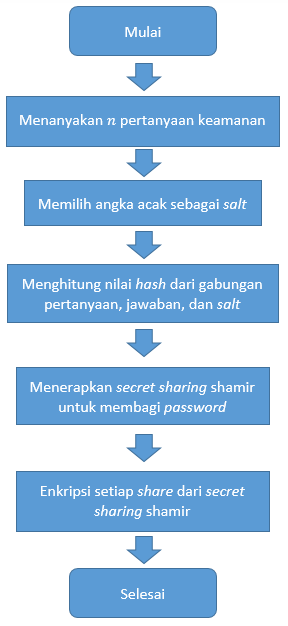
\includegraphics[scale=0.65]{Gambar/flowchart_share}}
	\caption{Proses pembangunan \textit{share} dari \textit{password}}\label{fig:create_share}
\end{figure}

Kemudian, untuk alur proses pembangunan kembali atau rekonstruksi \textit{password} dari \textit{share-share} yang ada ditunjukkan oleh Gambar \ref{fig:flowchart_reconstruct_secret}.

%diagram
\begin{figure}[H]
	\centerline{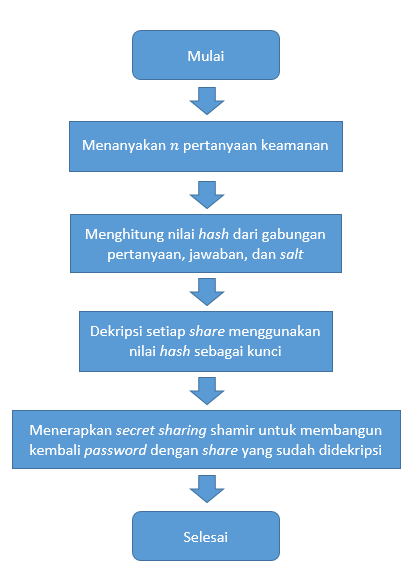
\includegraphics[scale=0.65]{Gambar/flowchart_reconstruct}}
	\caption{Proses pembangunan kembali atau rekonstruksi \textit{password}}\label{fig:flowchart_reconstruct_secret}
\end{figure}

\subsection{Diagram \textit{Use Case}}

Perangkat lunak yang dibangun akan memiliki 2 fitur utama, yaitu menyimpan \textit{password} beserta pertanyaan keamanan yang sifatnya personal dan mengembalikan \textit{password}. Saat menyimpan \textit{password}, pengguna akan diminta untuk menambahkan pertanyaan keamanan yang sifatnya personal dan saat mengembalikan \textit{password}, pengguna akan diminta untuk menjawab pertanyaan keamanan yang sudah disimpan saat menyimpan \textit{password}. Gambar \ref{fig:use_case} menunjukkan diagram \textit{use case} dari perangkat lunak.

%diagram
\begin{figure}[H]
	\centerline{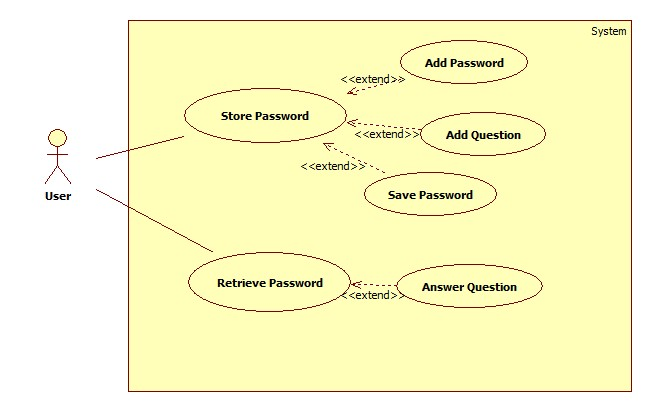
\includegraphics[scale=0.4]{Gambar/use_case}}
	\caption{Diagram \textit{use case} dari perangkat lunak}\label{fig:use_case}
\end{figure}

\subsection{Diagram Aktivitas}

Perangkat lunak yang dibangun memiliki 2 proses, yaitu menyimpan \textit{password} atau \textit{secret} dan mengembalikan \textit{password} atau \textit{secret}. Gambar \ref{fig:sharing-secret} menunjukkan diagram aktivitas untuk proses menyimpan \textit{password} atau \textit{secret}.

%diagram
\begin{figure}[H]
	\centerline{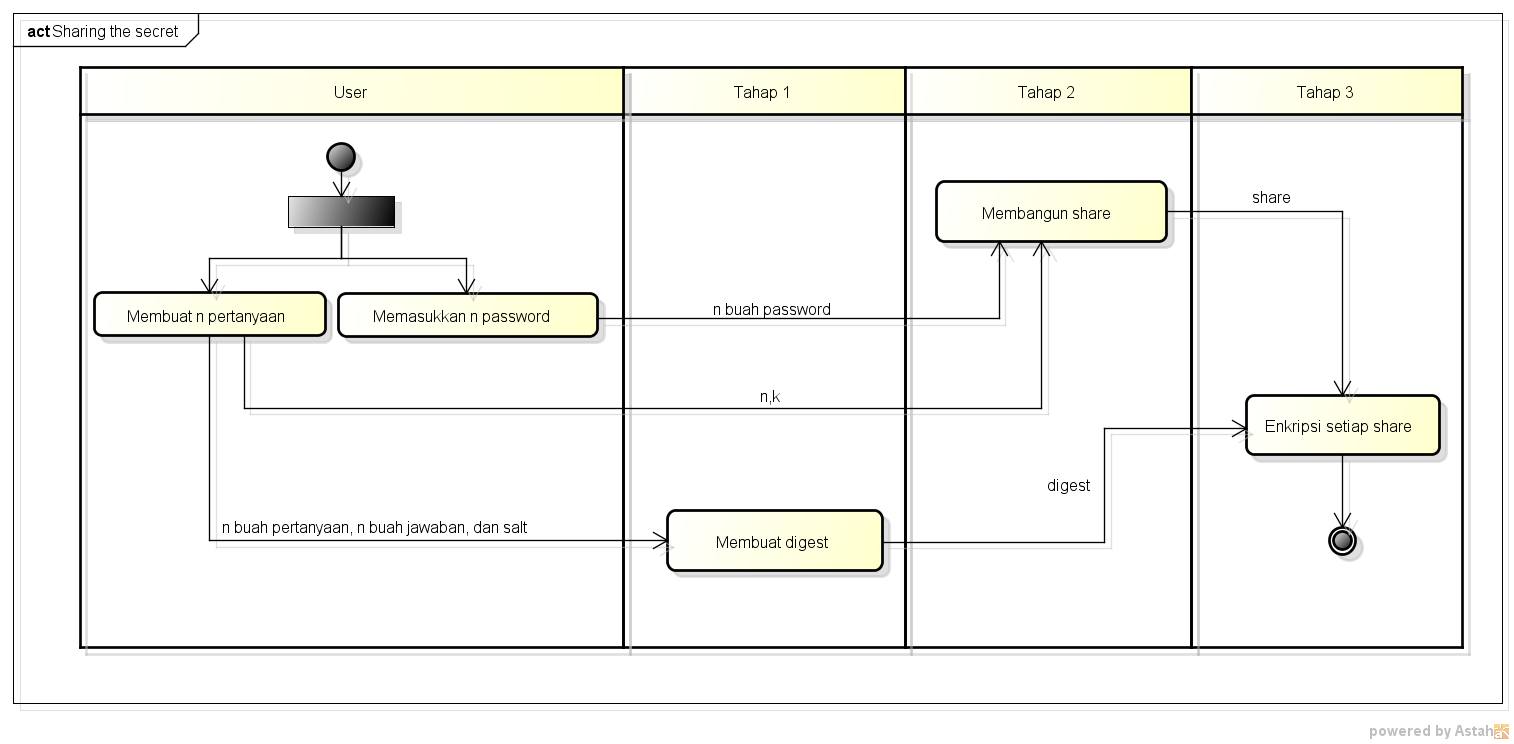
\includegraphics[scale=0.4]{Gambar/sharing-secret}}
	\caption{Diagram aktivitas untuk menyimpan \textit{password}}\label{fig:sharing-secret}
\end{figure}

Dalam proses menyimpan \textit{password}, awalnya \textit{user} harus terlebih dahulu menentukan banyak pertanyaan keamanan yang hendak digunakan (\begin{math}n\end{math}) dan banyak minimal pertanyaan keamanan yang bisa dijawab dengan benar untuk memeperoleh kembali \textit{password} (\begin{math}k\end{math}). Kemudian, \textit{user} akan menentukan pertanyaan keamanan personal yang akan digunakan.

Pertanyaan keamanan ini nantinya akan kembali digunakan untuk memperoleh kembali \textit{password} yang hilang atau dilupakan. Kemudian, setelah \textit{user} memilih dan menjawab setiap pertanyaan keamanan, setiap pertanyaan keamanan ini akan dihitung nilai \textit{hash}nya. Selanjutnya dengan menggunakan skema \textit{threshold (k, n)} untuk membagi \textit{password} menjadi sebanyak \begin{math}n\end{math} \textit{share}. Setiap \textit{share} ini akan dienkripsi dengan kunci nilai \textit{hash}.

Selanjutnya adalah proses untuk mengembalikan \textit{password}. Gambar \ref{fig:reconstruct} menunjukkan diagram aktivitas untuk proses mengembalikan \textit{password}.

%diagram
\begin{figure}[H]
	\centerline{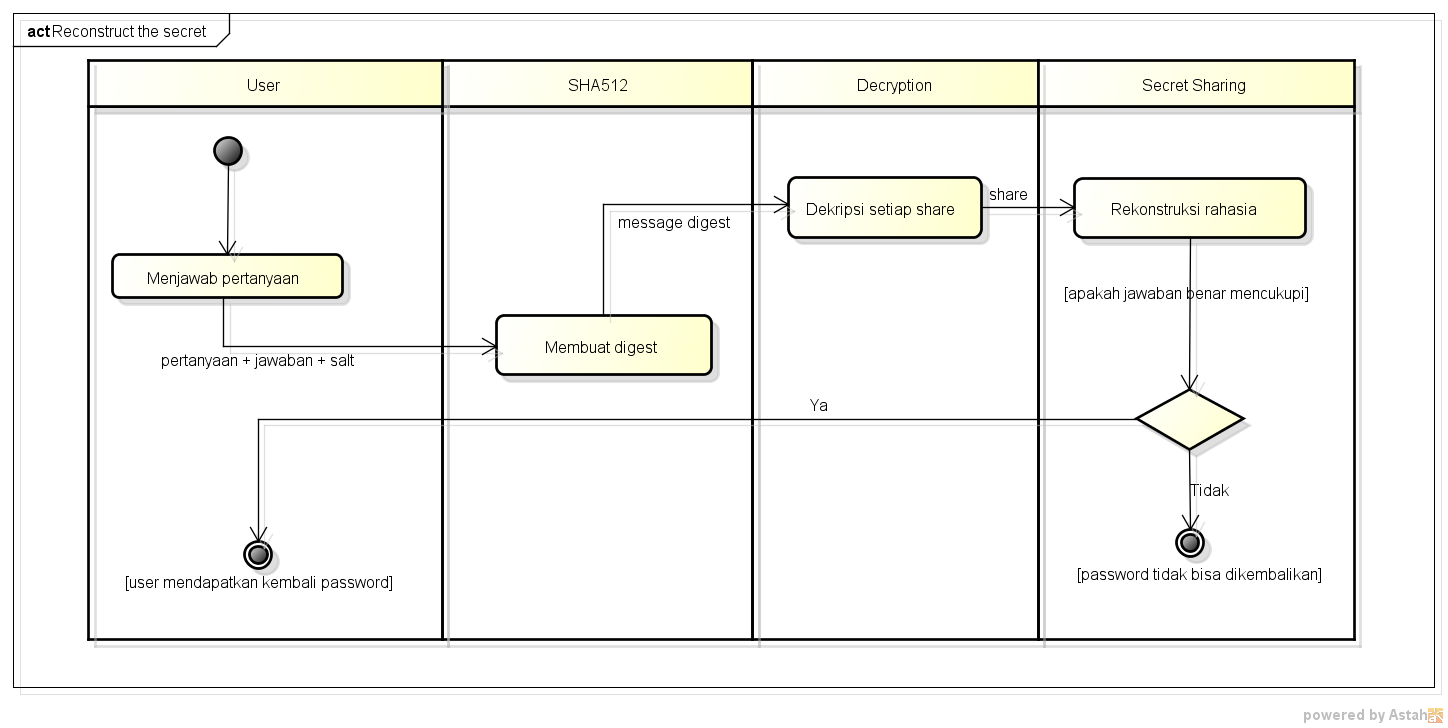
\includegraphics[scale=0.4]{Gambar/reconstruct-secret}}
	\caption{Diagram aktivitas untuk mengembalikan \textit{password}}\label{fig:reconstruct}
\end{figure}

Dalam proses untuk mengembalikan \textit{password}, \textit{user} akan diminta untuk menjawab beberapa pertanyaan keamanan yang sudah dipilih saat \textit{user} menyimpan \textit{password}. Selanjutnya adalah proses yang sama saat meyimpan \textit{password}, yaitu menghitung nilai \textit{hash} dari pertanyaan kemanan yang sudah dijawab oleh \textit{user}. Langkah selanjutnya adalah mendekripsi setiap \textit{share} dengan menggunakan kunci nilai \textit{hash}.

Langkah selanjutnya adalah dengan menggunakan skema \textit{threshold (k, n)} membangun atau rekontruksi ulang \textit{password}. Jika banyak pertanyaan yang dijawab benar oleh \textit{user} sama dengan atau lebih dari \begin{math}k\end{math} \textit{share}, maka \textit{user} bisa mendapatkan kembali \textit{password}, dan jika kurang dari \begin{math}k\end{math} \textit{share} maka \textit{user} tidak bisa mendapatkan kembali \textit{password}.

\subsection{Diagram Kelas}

Perangkat lunak yang dibangun memiliki 2 bagian utama, yaitu bagian \textit{engine} dan bagian antarmuka (\textit{user interface}). Bagian \textit{engine} berfungsi untuk menyimpan dan mengembalikan \textit{password}, melakukan proses enkripsi dan dekripsi, dan melakukan \textit{secret sharing}.

Bagian \textit{engine} merupakan sekumpulan kelas \textit{Java}, sedangkan bagian \textit{antarmuka} akan terdiri dari sekumpulan \textit{Java Server Page} atau JSP. Pada bagian ini akan dijelaskan bagian \textit{engine} saja. Gambar \ref{fig:diagramkelasengine} menunjukkan diagram kelas \textit{engine}.

%diagram
\begin{figure}[H]
	\centerline{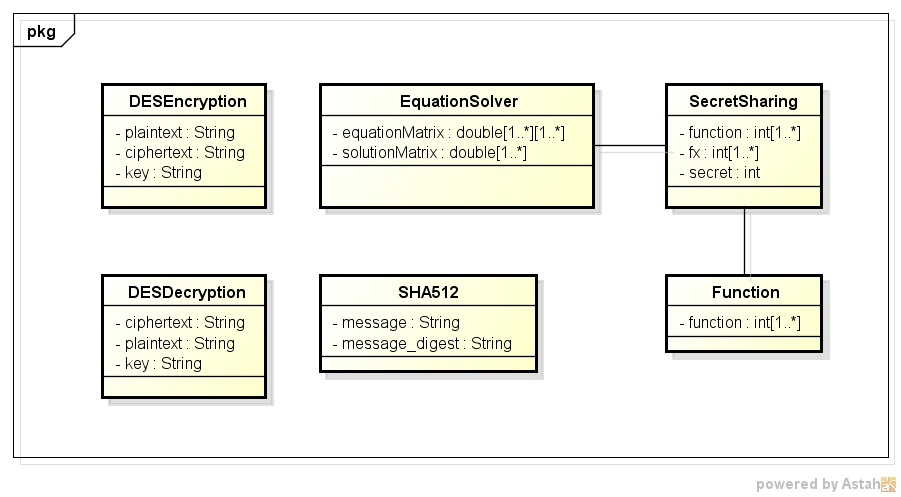
\includegraphics[scale=0.6]{Gambar/engine-class-diagram}}
	\caption{Diagram kelas \textit{engine}}\label{fig:diagramkelasengine}
\end{figure}

Untuk proses penyimpanan \textit{password}, kelas SHA512 berfungsi untuk menghitung nilai \textit{hash} dari gabungan pertanyaan, jawaban, dan \textit{salt}. Selanjutnya, kelas SecretSharing akan membagi \textit{password} menjadi beberapa \textit{share}. Kemudian, kelas DESEncryption akan mengenkripsi setiap \textit{share} dengan nilai \textit{hash} sebagai kunci rahasia. Setiap \textit{ciphertext} hasil enkripsi, nilai \textit{salt}, dan pertanyaan akan disimpan.

Untuk proses pengembalian \textit{password}, kelas SHA512 akan menghitung nilai \textit{hash} dari gabungan pertanyaan, jawaban, dan \textit{salt}. Kemudian, kelas DESDecryption akan mendekripsi \textit{ciphertext} hasil enkripsi yang disimpan dan kunci rahasia dari nilai \textit{hash} untuk memperoleh \textit{plaintext}. Kelas SecretSharing akan merekontruksi \textit{password} berdasarkan hasil dekripsi dari kelas DESDecryption. Jika, banyak pertanyaan benar sesuai, maka \textit{password} bisa dikembalikan.

\subsection{Arsitektur Perangkat Lunak}

Pada bagian sebelumnya sudah dijelaskan mengenai alur proses, diagram \textit{use case}, diagram aktivitas, dan diagram kelas dari perangkat lunak yang dibangun. Pada bagian ini akan dijelaskan mengenai seluruh bagian perangkat lunak yang dibangun. Seperti yang sudah dijelaskan sebelumnya perangkat lunak yang dibangun memiliki 2 bagian utama, yaitu bagian \textit{engine} dan bagian antarmuka. Gambar \ref{fig:arsitektur-perangkat-lunak} menunjukkan arsitektur dari perangkat lunak.

%diagram
\begin{figure}[H]
	\centerline{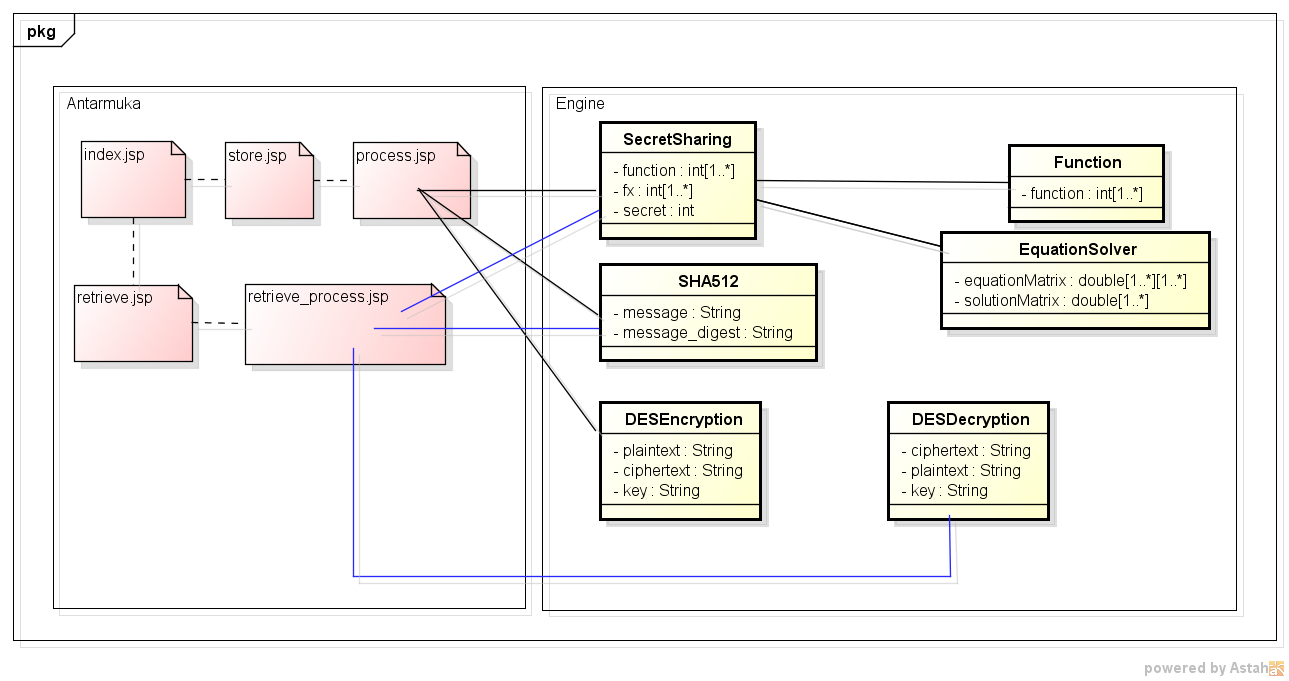
\includegraphics[scale=0.5]{Gambar/arsitektur}}
	\caption{Arsitektur perangkat lunak}\label{fig:arsitektur-perangkat-lunak}
\end{figure}

Untuk proses penyimpanan \textit{password}, sama seperti pada bagian sebelumnya, kelas yang akan digunakan adalah kelas SHA512 untuk menghasilkan \textit{hash}, kemudian kelas SecretSharing untuk menghasilkan \textit{share} dari \textit{password}, dan kelas DESEncryption untuk mengenkripsi masing-masing dari \textit{share} dengan nilai \textit{hash} sebagai kunci rahasia.

Selanjutnya, untuk proses pengembalian \textit{password}, kelas SHA512 akan digunakan kembali untuk menghasilkan \textit{digest}. Setelah \textit{digest} dihasilkan, kelas DESDecryption akan mendekripsi \textit{share-share} yang dimiliki dengan kunci \textit{digest} yang dihasilkan. Selanjutnya, kelas SecretSharing akan merekonstruksi ulang hasil dekripsi dari kelas DESDecryption dan menentukan apakah \textit{password} bisa dikembalikan atau tidak.